% $HeadURL$

\subsection{Glyph: \glyph{Unit of information}}
\label{sec:unitInfo}

When representing biological entities, it is often necessary to convey some abstract information about the entity's function that cannot (or does not need to) be easily related to its structure.
The \glyph{unit of information} is a decoration that can be used in this situation to add information to a glyph.
Some example uses include: characterising a logical part of an entity such as a functional domain (a binding domain, a catalytic site, a promoter, etc.), or the information encoded in the entity (an exon, an open reading frame, etc.).
A \glyph{unit of information} can also convey information about the physical environment, or the specific type of biological entity it is decorating.

\begin{glyphDescription}

\glyphSboTerm
Not applicable.


\glyphIncoming
None.



\glyphOutgoing
None.


\glyphContainer
A \glyph{unit of information} is represented by a rectangular shape, as shown in \fig{unitInfo}.


The centre of the shape should be placed on the border of the \glyph{EPN}.
% 

\glyphLabel
A \glyph{unit of information} is identified by a label that is  a string of characters that may be distributed on several lines to improve readability.
The centre of the label must be placed on the centre of the container.
The label may extend outside of the container.
  
For certain predefined types of information having controlled vocabularies associated with them, SBGN defines specific prefixes that must be included in the text of the label and associated with the information's value to indicate the type of information in question. Together, a prefix and a value constitute the label. The controlled vocabularies predefined in \SBGNPDLone are described in \sect{CVs} and summarised in the following list:

\begin{center}
  \begin{itemize}\setlength{\parskip}{0ex}
  \item[\texttt{pc}] container physical characteristic
  \item[\texttt{mt}] entity pool material type
  \item[\texttt{ct}] entity pool conceptual type
  \item[\texttt{N}]  multimer cardinality
  \end{itemize}
  
\end{center}

\glyphAux
None.

\end{glyphDescription}

\begin{figure}[H]
  \centering
  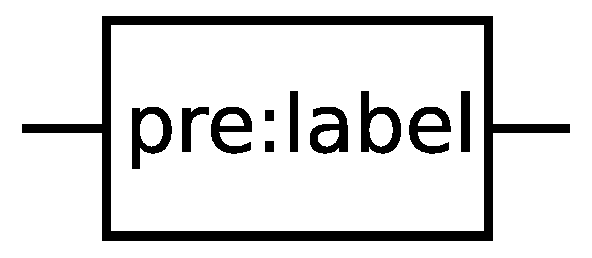
\includegraphics{images/unitInformation}
  \caption{The \PD glyph for \glyph{unit of information}, shown plain on the left, and decorating a \glyph{macromolecule} (\sect{macromolecule}) on the right.}
  \label{fig:unitInfo}
\end{figure}

% The following is for [X]Emacs users.   Please leave in place.
% Local Variables:
% TeX-master: "../sbgn_PD-level1"
% End:
